\documentclass{article}

\usepackage{amsmath, amsthm, amssymb, amsfonts}
\usepackage{thmtools}
\usepackage{graphicx}
\usepackage{setspace}
\usepackage{geometry}
\usepackage{float}
\usepackage{hyperref}
\usepackage[utf8]{inputenc}
\usepackage[english]{babel}
\usepackage{framed}
\usepackage[dvipsnames]{xcolor}
\usepackage{tcolorbox}
\usepackage{pgfplots}
\pgfplotsset{compat=1.17}
\usepackage{tikz}

\newcommand{\HRule}[1]{\rule{\linewidth}{#1}}

\newtheorem{axiom}{Axiom}[section] % a basic assumption about a mathematical situation
\newtheorem{definition}{Definition}[section] % an explanation of the mathematical meaning of a word
\newtheorem{notation}{Notation}[section] % an equivalent manifestation introduced to simplify mathematical writings
\newtheorem{theorem}{Theorem}[section] % a statement that has been proven to be true
\newtheorem{proposition}[theorem]{Proposition} % a less important but nonetheless interesting true statement
\newtheorem{corollary}{Corollary}[theorem] % a true statment that is a simple deduction from a theorem or proposition
\newtheorem{property}{Property}[theorem] % an obvious conclusion deducted from a theorem or proposition
\newtheorem{lemma}[theorem]{Lemma} % a less important theorem that is helpful in proving other true statements
\newtheorem{conjecture}{Conjecture}[section] % a statement believed to be true, but not yet proved
\newtheorem{example}{Example}[section]


\setstretch{1.2}
\geometry{
    textheight=9in,
    textwidth=5.5in,
    top=1in,
    headheight=12pt,
    headsep=25pt,
    footskip=30pt
}

% ------------------
\begin{document}
% ------------------
% Cover Page and ToC
% ------------------
\title{ \normalsize \textsc{}
		\\ [2.0cm]
		\HRule{1.5pt} \\
		\LARGE \textbf{\uppercase{Linear Algebra}
		\HRule{2.0pt} \\ [0.6cm] \vspace*{10\baselineskip}}}

\date{}
\author{\textbf{Author:} Nicholas Han \\ Shenyang 2025}

\maketitle
\thispagestyle{empty}
\newpage

\tableofcontents
\thispagestyle{empty}
\newpage
% ------------------


\pagenumbering{arabic}
\section{Linear Equations}

\begin{definition}[Linear Equation]
    A \textbf{linear equation} is an equation of variables of the first order. It may be put in the form of \(a_1x_1+a_2x_2+...+a_nx_n=b\), where \(x_1, x_2, ..., x_n\) are \textbf{variables} (or \textbf{unknowns}), \(a_1, a_2, ..., a_n\) are \textbf{coefficients}, and \(b\) is \textbf{constant}.
\end{definition}

\begin{definition}[System of Linear Equations]
    A \textbf{system of linear equations} (or a \textbf{linear system}) is a collection of one or more linear equations involving the same variables. It may be put in the form
    \begin{equation}\label{def_lin_eqn}
    \begin{split}
        a_{11}x_1+a_{12}x_2&+...+a_{1n}x_n=b_1,\\
        a_{21}x_1+a_{22}x_2&+...+a_{2n}x_n=b_2,\\
        &......\\
        a_{s1}x_1+a_{s2}x_2&+...+a_{sn}x_n=b_s\\
    \end{split}
    \end{equation}
    where \(a_{11}, a_{12}, ..., a_{sn}\) are \textbf{coefficients}, and \(b_1, b_2, ..., b_s\) are \textbf{constants}. And the number of equations \textbf{s} can be equal to, greater than, or less than the number of variables \textbf{n}.
\end{definition}

\begin{definition}[Solutions to a System of Linear Equations]
If there exist \(c_1, c_2, ..., c_n\) that can be plugged into \(x_1, x_2, ..., x_n\) so that the linear equations in (\ref{def_lin_eqn}) hold, the ordered list of \((c_1, c_2, ..., c_n)\) is called a \textbf{solution} to the system of linear equations. The set of all solutions is called the \textbf{solution set}.
\end{definition}

\subsection{The Geometry of Linear Equations}
Suppose we have a system of 2 linear equations with 2 variables.
    \begin{equation}\label{ex_lin_eqn}
    \begin{split}
    2x-y&=0 \\
    -x+2y&=3
    \end{split}
    \end{equation}
\subsubsection{Geometric Representation (by Rows)}
Each linear equation represents a line in the xy plane, and the intersection of the 2 lines (if there is one) represents the solution (in this case the only solution) to the system of equations, which is \(x=1\), \(y=2\).

\begin{center}
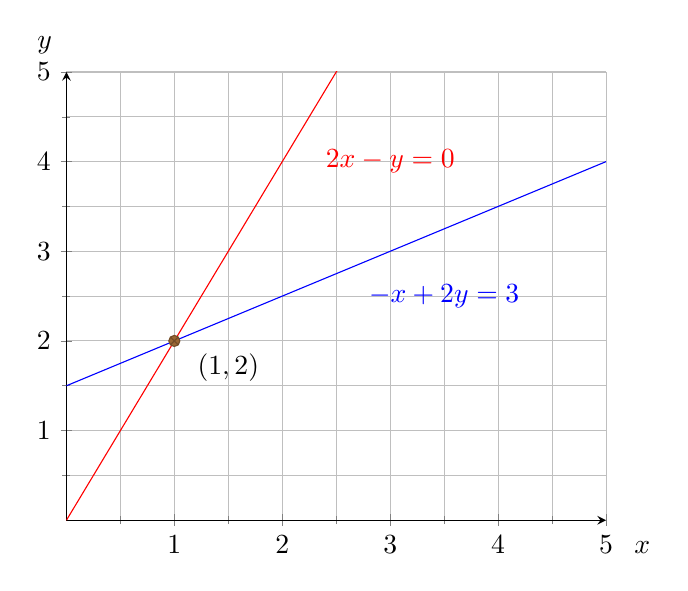
\begin{tikzpicture}
    \begin{axis}[grid=both,ymin=0,ymax=5,xmin=0,xmax=5,minor tick num=1,axis lines = middle,xlabel=$x$,ylabel=$y$,label style ={at={(ticklabel cs:1.1)}}]
        \addplot[domain=0:5,color=red]{2*x};
        \addplot[domain=0:5,color=blue]{x/2+1.5};
        \addplot+[only marks] coordinates {(1,2)};
        \node[color=red] at (axis cs: 3,4) {$2x-y=0$};
        \node[color=blue] at (axis cs: 3.5,2.5) {$-x+2y=3$};
        \node[color=black] at (axis cs: 1.5,1.7) {$(1,2)$};
    \end{axis}
\end{tikzpicture}
\end{center}

This representation of linear equations corresponds to that of analytic geometry that we studied in high school.

\subsubsection{Vector Representation (by Columns)}
\begin{notation}[Column Vector] A column vector $\vec{x}$ consisting of \textbf{m} elements is denoted as
\begin{center}
    \begin{equation}\label{col_vec}
    \begin{split}
    \vec{x}=\begin{bmatrix} x_1 \\ x_2 \\ \vdots \\ x_n \end{bmatrix} \;
    \end{split}
    \end{equation}
\end{center}
\end{notation}

We can thus rewrite the linear equations in (\ref{ex_lin_eqn}) by turning the coefficients into column vectors.
\begin{center}
\begin{equation}
    x \begin{bmatrix} \phantom{-} 2 \\ -1 \end{bmatrix} + y \begin{bmatrix} -1 \\ \phantom{-} 2 \end{bmatrix} = \begin{bmatrix} 0 \\ 3 \end{bmatrix}
\end{equation}
\end{center}

We want to find numbers $x$ and $y$ so that $x$ copies of vector $\begin{bmatrix} \phantom{-} 2 \\ -1 \end{bmatrix}$ added to $y$ copies of vector $\begin{bmatrix} -1 \\ \phantom{-} 2 \end{bmatrix}$ equals to $\begin{bmatrix} 0 \\ 3 \end{bmatrix}$.

\begin{center}
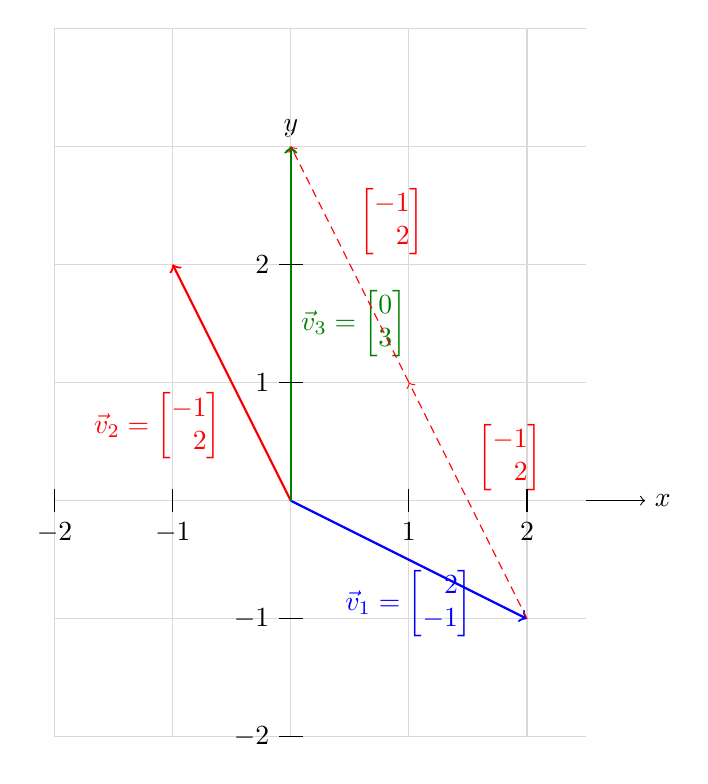
\begin{tikzpicture}[scale=1.5]
    % Draw coordinate axes
    \draw[->] (-2,0) -- (3,0) node[right] {$x$};
    \draw[->] (0,-2) -- (0,3) node[above] {$y$};
    
    % Draw grid
    \draw[gray!30] (-2,-2) grid (2.5,4);
    
    % Draw vectors
    \draw[->, thick, blue] (0,0) -- (2,-1) node[midway, below] {$\vec{v}_1 = \begin{bmatrix} \phantom{-} 2 \\ -1 \end{bmatrix}$};
    \draw[->, thick, red] (0,0) -- (-1,2) node[midway, below left] {$\vec{v}_2 = \begin{bmatrix} -1 \\ \phantom{-} 2 \end{bmatrix}$};
    \draw[->, thick, green!50!black] (0,0) -- (0,3) node[midway, right] {$\vec{v}_3 = \begin{bmatrix} 0 \\ 3 \end{bmatrix}$};
    \draw[->, densely dashed, red] (2,-1) -- (1,1) node[midway, above right] {$\begin{bmatrix} -1 \\ \phantom{-} 2 \end{bmatrix}$};
    \draw[->, densely dashed, red] (1,1) -- (0,3) node[midway, above right] {$\begin{bmatrix} -1 \\ \phantom{-} 2 \end{bmatrix}$};

    % Add some points for reference
    \foreach \x in {-2,-1,1,2}
        \draw (\x,0.1) -- (\x,-0.1) node[below] {$\x$};
    \foreach \y in {-2,-1,1,2}
        \draw (0.1,\y) -- (-0.1,\y) node[left] {$\y$};
\end{tikzpicture}
\end{center}

This representation of linear equations corresponds to that of vectors that we studied in high school.


\subsubsection{Matrix Representation}
Taking one more step forward, we write the linear equations in (\ref{ex_lin_eqn}) as a single equation using matrices and vectors.

\begin{center}
\begin{equation}
    \begin{bmatrix} \phantom{-} 2 -1 \\ -1 \phantom{-} 2 \end{bmatrix} \begin{bmatrix} x \\ y \end{bmatrix} = \begin{bmatrix} 0 \\ 3 \end{bmatrix}
\end{equation}
\end{center}

\begin{notation}[Matrix Representation]
    Given the linear equations (\ref{def_lin_eqn}), we denote the \textbf{coefficient matrix} as matrix
    $A = \begin{bmatrix}
        a_{11} \ a_{12} & ... \ a_{1n} \\
        a_{21} \ a_{22} & ... \ a_{2n} \\
        ...... \\
        a_{s1} \ a_{s2} & ... \ a_{sn} \\
    \end{bmatrix}$. The vector $\textbf{x}=\begin{bmatrix}x_1 \\ x_2 \\ ... \\ x_n \end{bmatrix}$ is the vector of unknowns. The values on the RHS of the equations are denoted as $\textbf{b}=\begin{bmatrix}b_1 \\ b_2 \\ ... \\ b_n \end{bmatrix}$. Thus, we have $A\textbf{x}=\textbf{b}$.
    
    
\end{notation}










\newpage
\section{Vector Space}
\begin{definition}[Binary Operation] Let $\mathbb{F}$ be a set. A binary operation is a function $\mathbb{F}$ $\times$ $\mathbb{F}$ $\rightarrow$ $\mathbb{F}$.
\end{definition}
\begin{example} Addition on real numbers is a binary operation.
\end{example}

\begin{definition}[Field] A Field $\mathbb{F}$ is a set together with two binary operations \textbf{addition} and \textbf{multiplication}, such that the following properties hold:
    \begin{equation}
    \begin{split}
    & \forall \alpha, \beta \in \mathbb{F}, \ \alpha+\beta=\beta+\alpha \ (additive \ commutativity) \\
    & \forall \alpha, \beta, \gamma \in \mathbb{F}, \ \alpha+(\beta+\gamma)=(\alpha+\beta)+\gamma \ (additive \ associativity) \\
    & \forall \alpha, \beta \in \mathbb{F}, \alpha \cdot \beta = \beta \cdot \alpha \ (multiplicative \ commutativity) \\
    & \forall \alpha, \beta, \gamma \in \mathbb{F}, \ \alpha \cdot (\beta \cdot \gamma)=(\alpha \cdot \beta) \cdot \gamma \ (multiplicative \ associativity) \\
    & \forall \alpha, \beta, \gamma \in \mathbb{F}, \alpha \cdot (\beta + \gamma)=\alpha \cdot \beta + \alpha \cdot \gamma \ (distributivity) \\
    \end{split}
    \end{equation}
\end{definition}

% ------------------
% Reference and Cited Works
% ------------------

\bibliography{References.bib}

% ------------------

\bibliographystyle{IEEEtran}

\end{document}
